
\subsection{Producing the activity plan}

After the app generates the dataset of POIs and the
user's travel interest vector, we formulate an
efficient activity plan using these two inputs. This
itinerary generator is based on the existing state of
the art activity planners~\cite{Sylejmani2017, Wisittipanich2020}
with some adjustments: We wanted the trip's output to take the
form of an itinerary.  The problem takes the form of
the `day' and `night'  category split discussed in
the literature review.  The scoring of itineraries is adjusted
with the travel interest vector.

The problem definition of our novel itinerary planner
is mathematically formulated as follows. A tourist trip is made up
of some pre-defined user constants alongside the travel interest
vector. The predefined constants are:
\\


\setlength{\tabcolsep}{20pt}

\begin{tabular}{l l}

\textit{M}:  &  The number of travelling days \\
\textit{C}: & The activity pace (ie. the greater the \\
 & C value, the more activities are generated in \\
 & a day) \\  
\end{tabular}
\\
\\
\\
The objective function of our itinerary planner is:

\[ \text{MAX}  \sum_{m=0}^{M} ( S_{{D_m}} + S_{{E_m}}) \]
where:
\\
\begin{tabular}{l l}
% \textit{i,j}:  &  POI (\textit{i,j} = 2,3,...,\textit{N}) \\
\textit{m} & Travelling day (\textit{m}=1,2,\ldots, textit{M}) \\ 
\textit{$D_m$} & Morning section of day number m \\  
\textit{$E_m$} & Evening section of day number m \\  
\textit{$S_{D_m}$} & Score of the morning section $D_m$ \\  
\textit{$S_{E_m}$} & Score of the evening section $E_m$ \\  
\end{tabular}
\\
\\

A day is made up of the morning ${D_m}$ section and
the evening ${E_m}$ section. The timetable suggests a
POI in the morning, then somewhere to eat, and the
rest is dependant on the activity pace C. That is why
the morning section is made up of $C + 2$ tourist
attractions. The evening section suggests a place to
eat and a POI; therefore, the evening section is just
made up of $2$. 


\[D_m = Y_i + Y_f + C ( Y_i) \]
\[E_m = Y_f + Y_j \]

\begin{tabular}{l l}

\textit{i} & Morning Tourist attraction (i = 1, 2, 3,…, $n_1$)\\
\textit{j} & Evening Tourist attraction (j = 1,2, 3,…, $n_2$)\\
\textit{f} & Food Place (f = 1,2, 3,…, $n_3$)\\
\textit{$Y_{i|f|j}$}: & 1 if a tourist visit attraction i, j or f and  0 if otherwise\\
\end{tabular}
\\ 
\\
\begin{tabular}{l l}
\textbf{Constraints} & \\
\textit{$ \sum_{m=0}^{M}\sum_{i=0}^{n_1}{Y_i} \leq 1$} & Ensures that all morning tourist attractions are \\ & not visited more than once throughout the whole \\ & itinerary\\

\textit{$ \sum_{m=0}^{M}\sum_{j=0}^{n_1}{Y_j} \leq 1$} & Ensures that all evening tourist attractions are \\ & not visited only once throughout the whole \\ & itinerary\\


\end{tabular}

\subsubsection{Calculation of Score}

The score $S_{D_m}$ or $S_{E_m}$ is calculated using

\[ S_{D_m | E_m} = \frac{1}{T} + R + V\]

where:
\\
\begin{tabular}{l l}
% \textit{i,j}:  &  POI (\textit{i,j} = 2,3,...,\textit{N}) \\
\textit{T} & Total distance between each tourist attractions in the \\ & morning/evening of day m\\ 
\textit{R} & Average rating of the tourist attractions in the \\ & morning/evening of day m \\  
\textit{V} & how much the tourist attractions of the \\ & morning/evening of day m match with the user's \\ & travel interest vector \\  

\end{tabular}
\\
\\


\subsubsection{Particle Swarm optimisation algorithm}

%TODO: Short description of PSO PSO with bias randomisation
%Flow-chart/algorithm

Kennedy et al.~\cite{Kennedy} proposed the original PSO algorithm in
1995 designed to solve optimisation problems. The
algorithm is a population-based technique that uses \textit{n}
elements called particles. Each particle has a
d-dimensional \textit{position} vector representing a solution
and a d-dimensional \textit{velocity} vector expressing the
direction of the particle during its search period. 

When a PSO program initialises all of the particles,
they are usually set to a random or predetermined
value. In our algorithm, we introduce a method of
randomisation bias. Although the initial particles are
generated randomly, the randomness is weighted and
affected by three things: 
\begin{enumerate}
    
    \item The user's travel interest vector 
    \item the place's rating 
    \item the place's number of ratings.

\end{enumerate}
  We implemented the randomness bias to give a
head start to the algorithm rather than just starting
optimising from purely random itineraries. Figure X
shows an example of a sample place with its
probability of being chosen as part of the initial
particles alongside a sample tourist interest vector.
At each iteration in the algorithm, the velocity of
each particle is calculated based on the inertia
constant and how well it is doing compared with its
personal best score and the global best score. The
inertia constant helps the particle explore new
solutions and escape the local minima. After a few
iterations have passed, particles use this velocity
and move towards the optimum position. We demonstrate
the framework of our PSO algorithm in Figure~\ref{FlowChart}.

\begin{figure}[h]
\centering
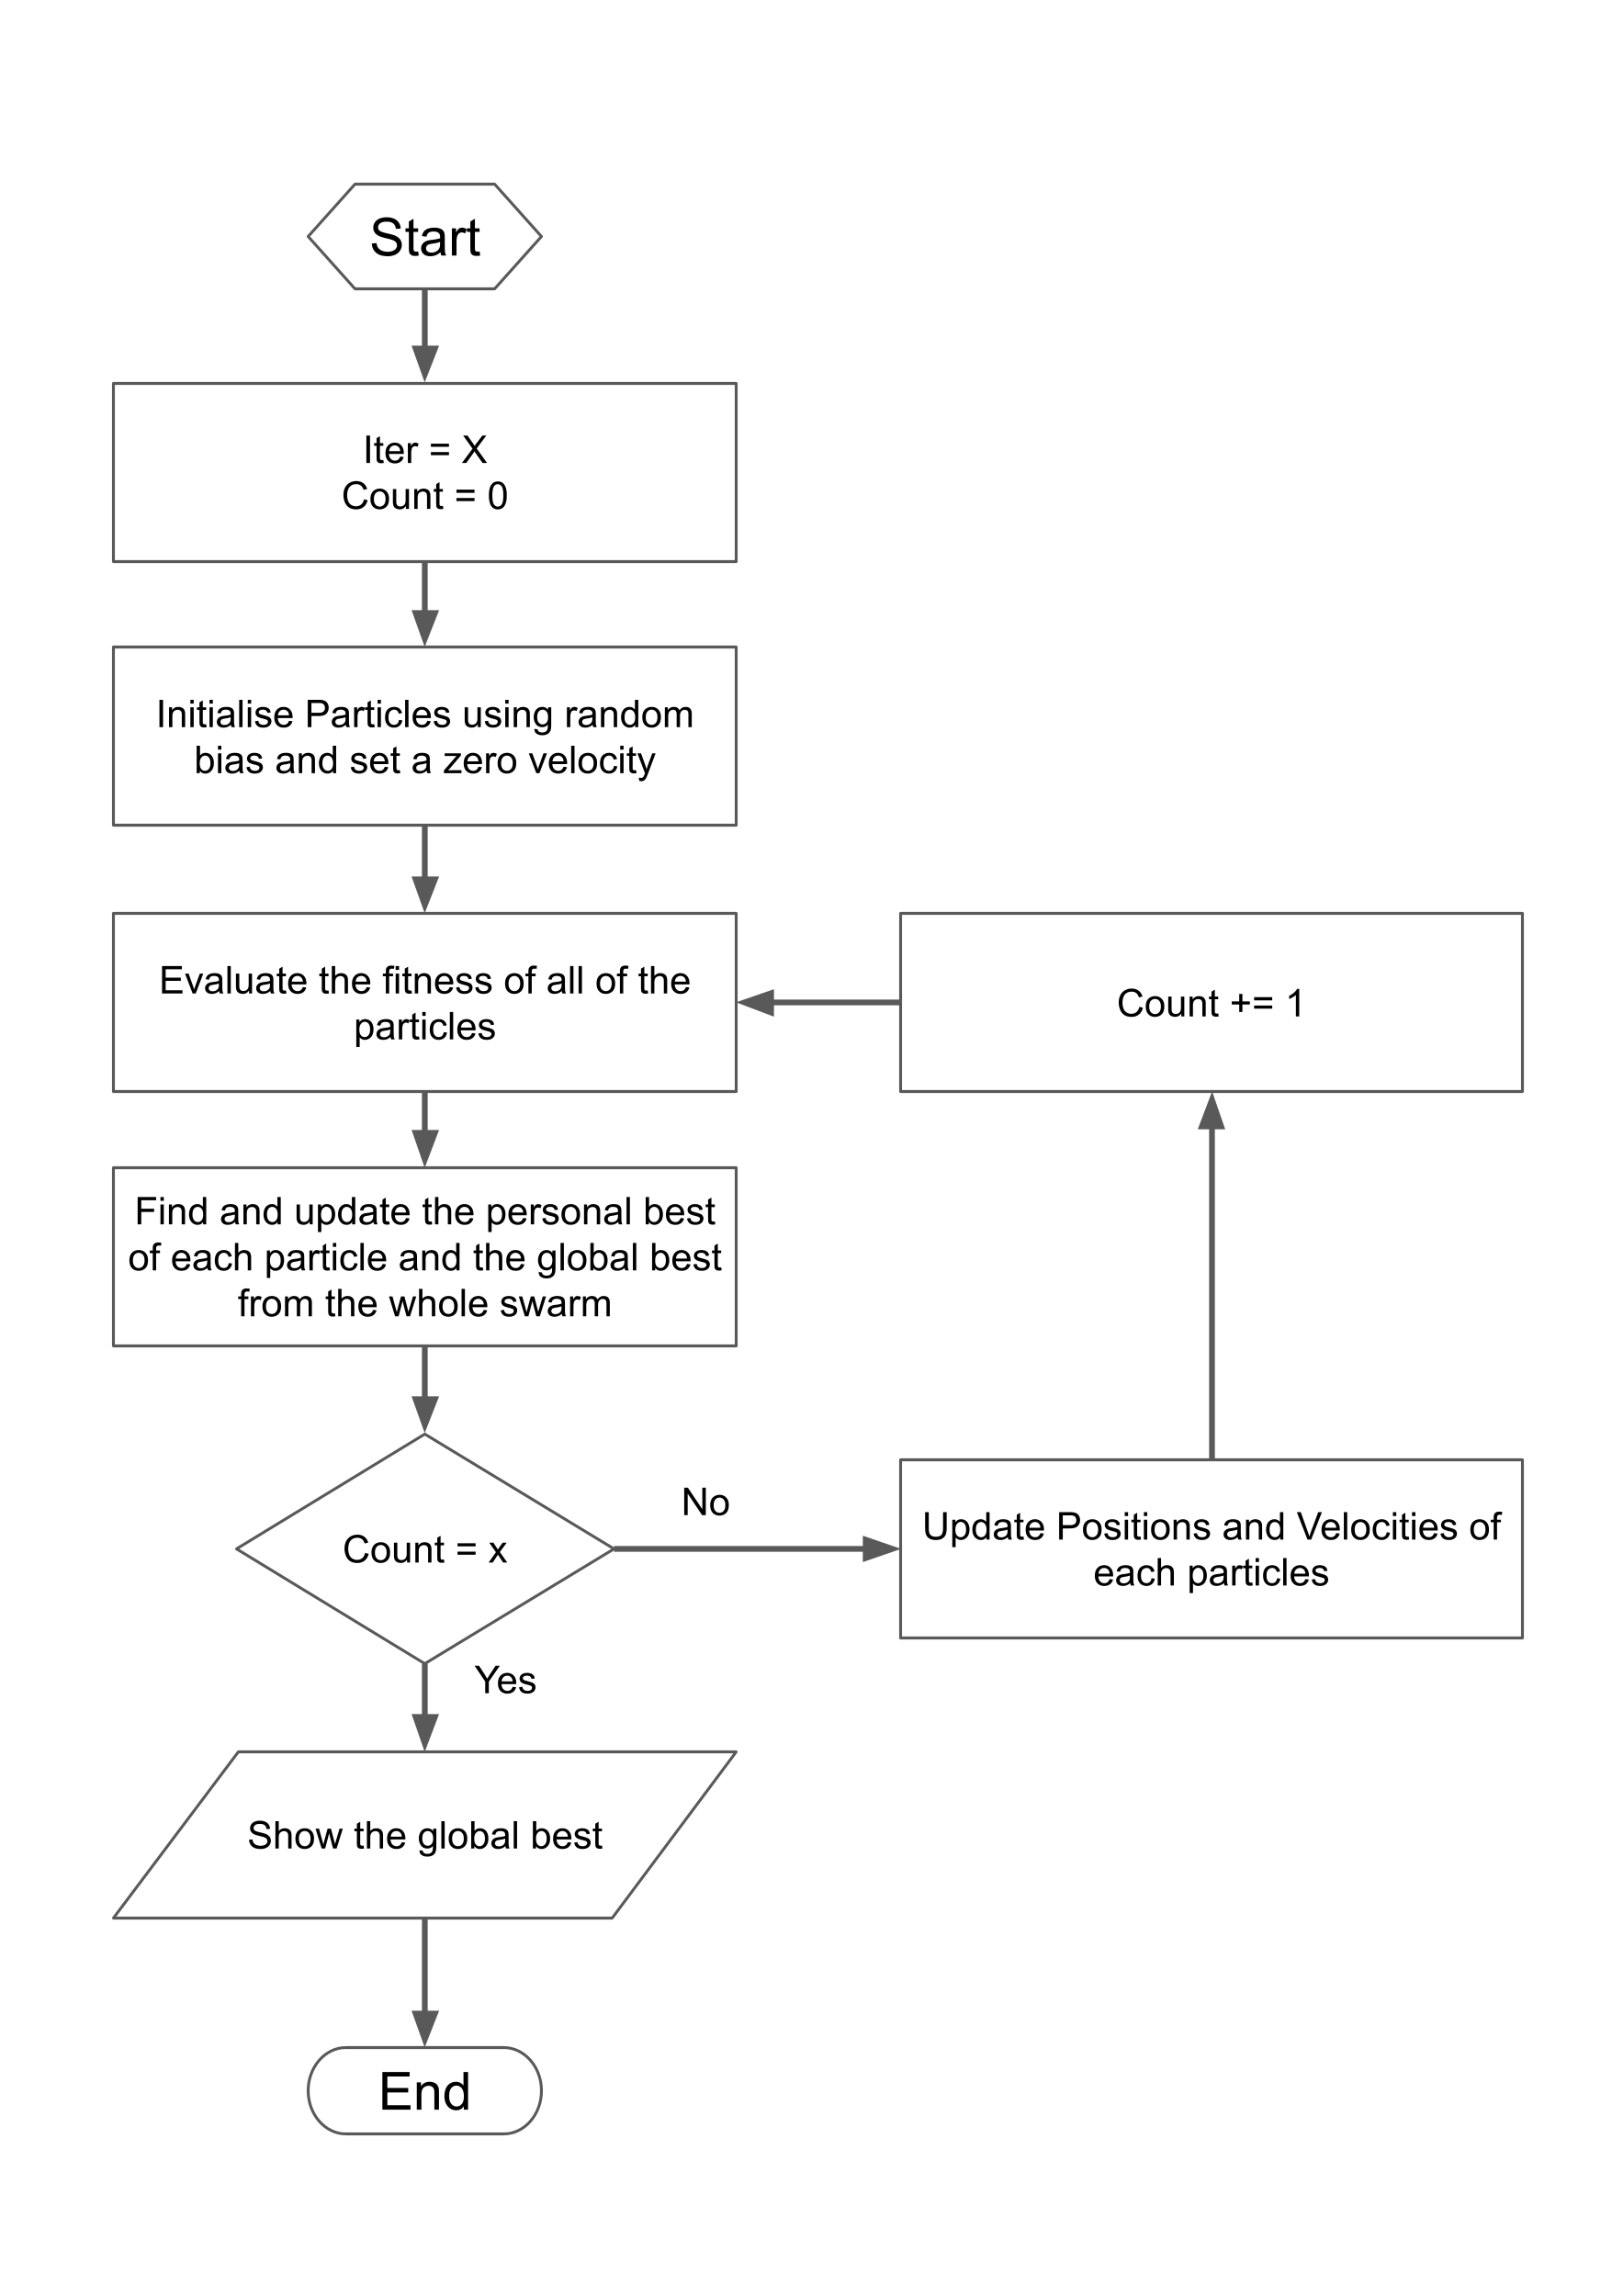
\includegraphics[width=0.5\textwidth]{FlowChart.png}
\caption{Framework of PSO algorithm}
\label{FlowChart}
\end{figure}

\subsection{Web application implementation and user
interface}

We built the application using several technologies
where each communicates with each other to provide a
user-friendly website for the potential tourist.
Figure~\ref{TechStack} shows the tech stack diagram of the website.
The website is accessible through the URL
\url{https://www.touristplanner.xyz}. We built the front end of the website using HTML, CSS and javascript and hosted it
on a cloud Vultr server. The website is 
responsive to be accessible from both a
mobile phone and a laptop. The website communicates
with the back end of the application using REST
endpoints, hosted on a separate dedicated server
provided by Hetzner using the Java Spring Boot
framework.  Another Python Gunicorn server is used to
generate the itinerary and calculate a travel interest
vector which sends the information directly to the
Spring boot server. Finally, a local instance of an
Open Source Routing Machine server calculates the
distances from one tourist attraction to another used
by the Gunicorn server to optimise the itinerary. 

\begin{figure}[h]
\centering
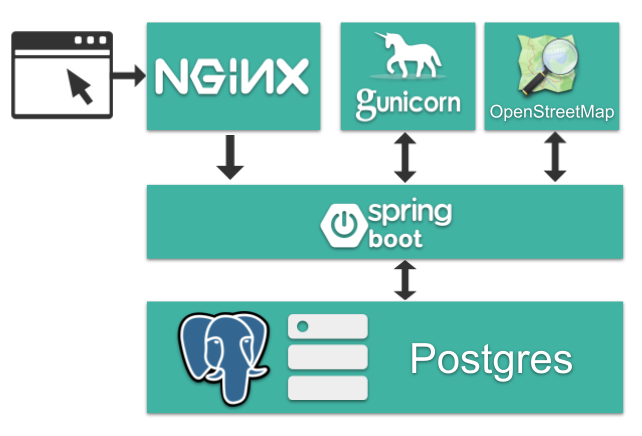
\includegraphics[width=0.5\textwidth]{TechStack.png}
\caption{Tech Stack implementation of the application}
\label{TechStack}
\end{figure}

\begin{figure}[h]
\centering
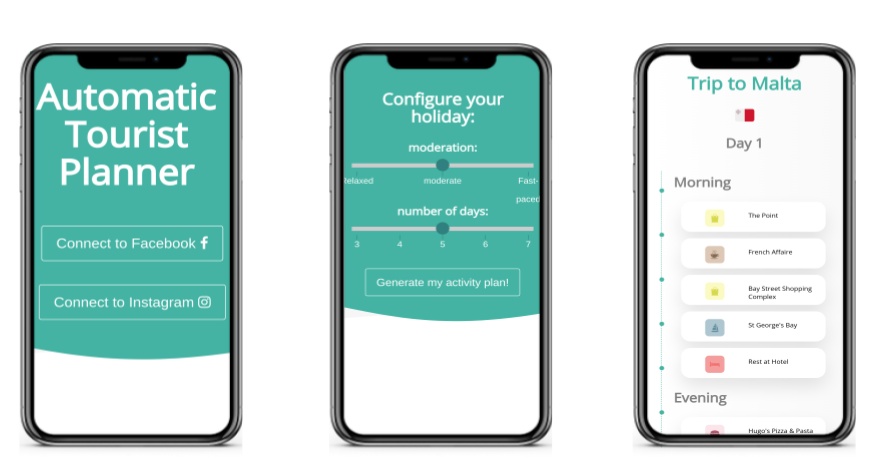
\includegraphics[width=0.7\textwidth]{Process.png}
\caption{User Experience Timeline}
\label{Timeline}
\end{figure}

Figure~\ref{Timeline} shows screenshots of the website portraying
the user's timeline.  The user navigates to the
homepage, accepts terms and conditions and connect his
social media profiles.  The user selects the number of
days M and the activity moderation C.  The website
navigates to the final page of the application
exhibiting their personalised itinerary. 
